%%%%%%%%%%%%%%%%%%%% book.tex %%%%%%%%%%%%%%%%%%%%%%%%%%%%%
%
% sample root file for the chapters of your "monograph"
%
% Use this file as a template for your own input.
%
%%%%%%%%%%%%%%%% Springer-Verlag %%%%%%%%%%%%%%%%%%%%%%%%%%


% RECOMMENDED %%%%%%%%%%%%%%%%%%%%%%%%%%%%%%%%%%%%%%%%%%%%%%%%%%%
\documentclass[graybox,envcountchap,sectrefs]{svmono}

% choose options for [] as required from the list
% in the Reference Guide

%\usepackage{mathptmx}
%\usepackage{helvet}
%\usepackage{courier}
%
\usepackage{type1cm}         

\usepackage{makeidx}         % allows index generation
\usepackage{graphicx}        % standard LaTeX graphics tool
                             % when including figure files
\usepackage{multicol}        % used for the two-column index
\usepackage[bottom]{footmisc}% places footnotes at page bottom

\usepackage{newtxtext}       % 
\usepackage{newtxmath}       % selects Times Roman as basic font

% see the list of further useful packages
% in the Reference Guide

\makeindex             % used for the subject index
                       % please use the style svind.ist with
                       % your makeindex program

%%%%%%%%%%%%%%%%%%%%%%%%%%%%%%%%%%%%%%%%%%%%%%%%%%%%%%%%%%%%%%%%%%%%%

\graphicspath{{./}{images/}}

\begin{document}

\author{Iddo Tzameret}
\title{Introduction to Concrete Complexity}
\subtitle{Lecture Notes \\ 
\normalsize{Imperial College London} \\ \normalsize{Dept. of Computing}
}
\maketitle

\frontmatter%%%%%%%%%%%%%%%%%%%%%%%%%%%%%%%%%%%%%%%%%%%%%%%%%%%%%%

%
%%%%%%%%%%%%%%%%%%%%%%% dedic.tex %%%%%%%%%%%%%%%%%%%%%%%%%%%%%%%%%
%
% sample dedication
%
% Use this file as a template for your own input.
%
%%%%%%%%%%%%%%%%%%%%%%%% Springer %%%%%%%%%%%%%%%%%%%%%%%%%%

\begin{dedication}
Use the template \emph{dedic.tex} together with the Springer document class SVMono for monograph-type books or SVMult for contributed volumes to style a quotation or a dedication\index{dedication} at the very beginning of your book
\end{dedication}





%%%%%%%%%%%%%%%%%%%%%%%foreword.tex%%%%%%%%%%%%%%%%%%%%%%%%%%%%%%%%%
% sample foreword
%
% Use this file as a template for your own input.
%
%%%%%%%%%%%%%%%%%%%%%%%% Springer %%%%%%%%%%%%%%%%%%%%%%%%%%

\foreword

%% Please have the foreword written here
Use the template \textit{foreword.tex} together with the document class SVMono (monograph-type books) or SVMult (edited books) to style your foreword\index{foreword}. 

The foreword covers introductory remarks preceding the text of a book that are written by a \textit{person other than the author or editor} of the book. If applicable, the foreword precedes the preface which is written by the author or editor of the book.


\vspace{\baselineskip}
\begin{flushright}\noindent
Place, month year\hfill {\it Firstname  Surname}\\
\end{flushright}



%%%%%%%%%%%%%%%%%%%%%%%preface.tex%%%%%%%%%%%%%%%%%%%%%%%%%%%%%%%%%%%%%%%%%
% sample preface
%
% Use this file as a template for your own input.
%
%%%%%%%%%%%%%%%%%%%%%%%% Springer %%%%%%%%%%%%%%%%%%%%%%%%%%

\preface

%% Please write your preface here
Use the template \emph{preface.tex} together with the document class SVMono (monograph-type books) or SVMult (edited books) to style your preface.

A preface\index{preface} is a book's preliminary statement, usually written by the \textit{author or editor} of a work, which states its origin, scope, purpose, plan, and intended audience, and which sometimes includes afterthoughts and acknowledgments of assistance. 

When written by a person other than the author, it is called a foreword. The preface or foreword is distinct from the introduction, which deals with the subject of the work.

Customarily \textit{acknowledgments} are included as last part of the preface.
 

\vspace{\baselineskip}
\begin{flushright}\noindent
Place(s),\hfill {\it Firstname  Surname}\\
month year\hfill {\it Firstname  Surname}\\
\end{flushright}



%%%%%%%%%%%%%%%%%%%%%%%acknow.tex%%%%%%%%%%%%%%%%%%%%%%%%%%%%%%%%%%%%%%%%%
% sample acknowledgement chapter
%
% Use this file as a template for your own input.
%
%%%%%%%%%%%%%%%%%%%%%%%% Springer %%%%%%%%%%%%%%%%%%%%%%%%%%

\extrachap{Acknowledgements}

%Use the template \emph{acknow.tex} together with the document class SVMono (monograph-type books) or SVMult (edited books) if you prefer to set your acknowledgement section as a separate chapter instead of including it as last part of your preface.



Let me acknowledge the following who have sent typos, corrections and suggestions for  the preliminary drafts of this manuscript.

Thom Hughes and Yu Xuanyu.

Special thanks to Michal Garlik for discussions, ideas and his notes related to this manuscript. 



\tableofcontents

%%%%%%%%%%%%%%%%%%%%%%%acronym.tex%%%%%%%%%%%%%%%%%%%%%%%%%%%%%%%%%%%%%%%%%
% sample list of acronyms
%
% Use this file as a template for your own input.
%
%%%%%%%%%%%%%%%%%%%%%%%% Springer %%%%%%%%%%%%%%%%%%%%%%%%%%

\extrachap{Acronyms}

Use the template \emph{acronym.tex} together with the document class SVMono (monograph-type books) or SVMult (edited books) to style your list(s) of abbreviations or symbols.

Lists of abbreviations\index{acronyms, list of}, symbols\index{symbols, list of} and the like are easily formatted with the help of the Springer-enhanced \verb|description| environment.

\begin{description}[CABR]
\item[ABC]{Spelled-out abbreviation and definition}
\item[BABI]{Spelled-out abbreviation and definition}
\item[CABR]{Spelled-out abbreviation and definition}
\end{description}


\mainmatter%%%%%%%%%%%%%%%%%%%%%%%%%%%%%%%%%%%%%%%%%%%%%%%%%%%%%%%
%%%%%%%%%%%%%%%%%%%%%%part.tex%%%%%%%%%%%%%%%%%%%%%%%%%%%%%%%%%%
% 
% sample part title
%
% Use this file as a template for your own input.
%
%%%%%%%%%%%%%%%%%%%%%%%% Springer %%%%%%%%%%%%%%%%%%%%%%%%%%

\begin{partbacktext}
\part{Part Title}
\noindent Use the template \emph{part.tex} together with the document class SVMono (monograph-type books) or SVMult (edited books) to style your part title page and, if desired, a short introductory text (maximum one page) on its verso page.

\end{partbacktext}
%%%%%%%%%%%%%%%%%%%%% chapter1.tex %%%%%%%%%%%%%%%%%%%%%%%%%%%%%%%%%
%
%  
%
% Use this file as a template for your own input.
%
%%%%%%%%%%%%%%%%%%%%%%%% Springer-Verlag %%%%%%%%%%%%%%%%%%%%%%%%%%
%\motto{Use the template \emph{chapter.tex} to style the various elements of your chapter content.}






\section{Summary of Module}
\label{sec:1}

 We are interested in approaches to the fundamental hardness questions in computational complexity.

Computational complexity: the study of which problems can be efficiently computed and which cannot.

Efficiency: we understand efficiency as Polynomial Time computability. A Boolean function $f:\{0,1\}^n\to\{0,1\}$ is said to be efficiently computable if there is a polynomial-time Turing Machine M that, on input $x$ in $\bits^n$ outputs $f(x)$ and runs in time $n^c$ for some constant $c$. Note that $n^c$ is a polynomial in the input length $n$ (the exponent $c$ does not depend on the input length $n$). 

The arguably main question of the theory of computation, the one that subsumes in some sense many problems in other parts of computing, once is the \P~vs~\NP~question: Can we separate \P~from \NP, namely, is there a language in \NP~ that is not in \P? In other words, can we prove that SAT (Boolean satisfiability problem) cannot be solved in polynomial time? And yet again, roughly, can problems whose solutions once given can be verified efficiently, can be solved efficiently? 

We are interested in \emph{concrete} approaches, namely, considering a simple, usually combinatorial-looking, model of computation, such as a Boolean circuit, and establishing lower bounds against the size of circuits required to prove certain specific functions that are given to us concretely (usually, these functions also possess some straightforward combinatorial 
properties; e.g., they represented specific graph problems). In this sense, the question is concrete because the result is unconditional (namely, it does not depend on unproved 
assumptions, such as $\P\neq\NP$), and the model itself is concrete: it is a (primarily combinatorial) object of which its size we lower 
bound in precise terms (e.g., circuit $C$ computing function $f(x)$ must have size $2^{|x|}$, where $|x|$ is the bit-size of the input $x$).
\medskip 

Three main concrete approaches to the fundamental hardness questions are the following:

\begin{enumerate}
\item  Circuit Complexity 
\item Proof Complexity 
\item Algebraic Complexity
\end{enumerate}

We shall see a bit from each, mainly circuit complexity and some basic proof complexity while commenting briefly on algebraic complexity. 



Other approaches to the fundamental hardness questions are usually more intrinsic to complexity theory. In that respect, the whole of computational complexity theory could be viewed as ``approaching" the fundamental hardness questions through complexity class, reductions, concrete lower bounds and the relation between these notions and results. One intriguing approach that makes this attempt in particular is the ``Meta Complexity" approach. We are not going to touch on this in this course. 



\chapter{Introduction to Circuit Complexity}
\label{intro} % Always give a unique label
% use \chaptermark{}
% to alter or adjust the chapter heading in the running head
 

\section{Basic Circuit Complexity}
\label{sec:2}
% Always give a unique label
% and use \ref{<label>} for cross-references
% and \cite{<label>} for bibliographic references
% use \sectionmark{}
% to alter or adjust the section heading in the running head

\begin{definition}[Boolean Circuit]
Let $n \in \mathbb{N}$ and $x_1, \ldots, x_n$ be $n$ variables. A Boolean Circuit $C$ with $n$ inputs is a directed acyclic graph. It contains $n$ nodes with no incoming edges, called the \emph{input nodes} and a single node with no outgoing edges, called the \emph{output node}.
All other nodes are \emph{internal nodes} or \emph{gates}, and
are labelled by the logical gates $\lor, \land,\neg$ (i.e., logical OR, AND, NOT, resp.). The $\lor,\land$ nodes have fan-in (i.e., number of incoming nodes) 2, and $\neg$ has fan-in 1. The \emph{size of $C$}, denoted $|C|$, is the number of nodes in the underlying graph.
$C$ is called a \emph{formula} if each node has at most one outgoing edge (i.e., the underlying graph is a tree),
\end{definition}




\begin{figure}
\sidecaption
  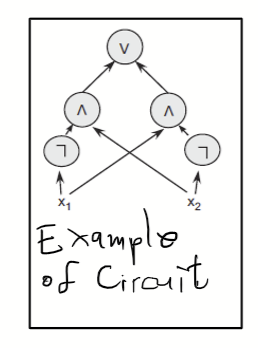
\includegraphics[width=0.2\linewidth]{images/Example-circuit.png}
    \caption{Example of a simple Boolean circuit.}
    \label{fig:enter-label}
\end{figure}

%
\begin{trailer}{Comment}
Fan-in $d>2$ 
can be simulated by a tree of $d-1 $ nodes: 
\begin{figure}[h]
    \centering
  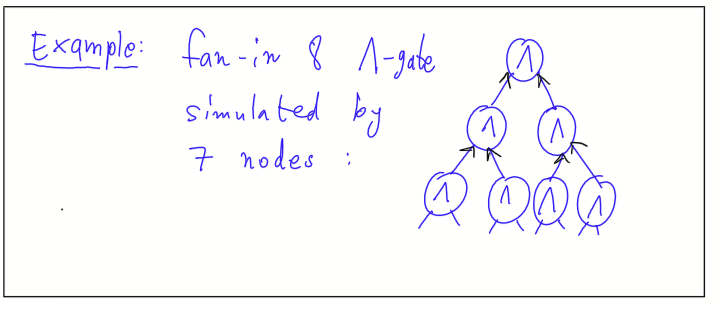
\includegraphics[width=0.5\linewidth]{images/Example-tree-circuit.png}
    \label{fig:enter-label}
\end{figure}
\end{trailer}


\newpage 

\begin{question}{What is the function computed by the circuit below?}
\begin{figure}
    \centering
    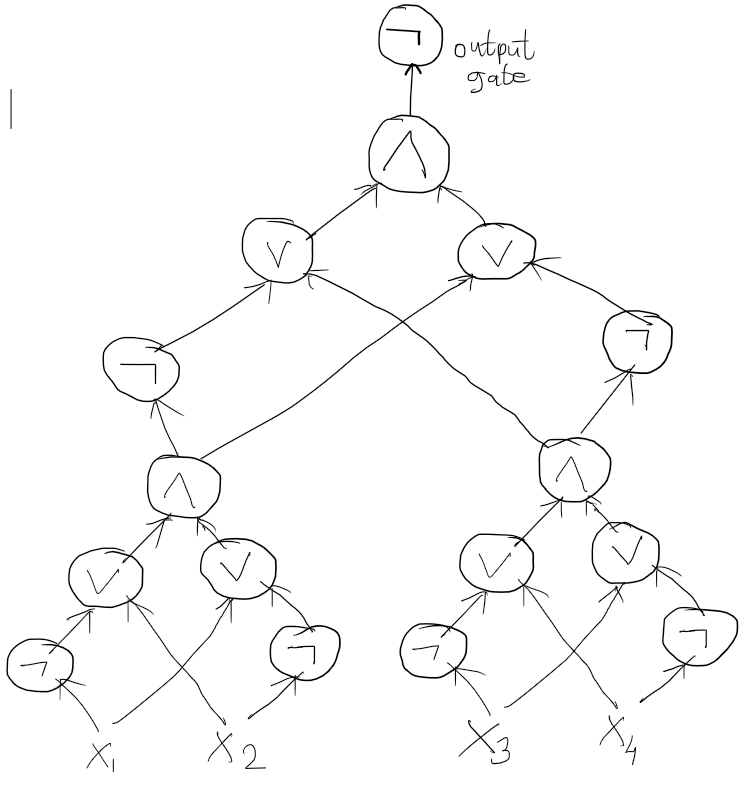
\includegraphics[width=0.75\linewidth]{images/parity-circuit-question.png}
    \caption{Question}
    \label{fig:enter-label}
\end{figure}
\end{question}

\begin{trailer}{Answer}
     PARITY on 4 input bits. It outputs 1 if the number of 1's in the input is odd. I.e., it computes the XOR of $x_1, \ldots, x_4$. In other words, it computes the function $x_1+x_2+x_3+x_4$ mod 2. (Understand why that is. Hint: recall that ${\neg x_1}\lor x_2$ is logically equivalent to $x_1\to x_2$. And notice that this structure repeats throughout the circuit.)
\end{trailer}
%\eject

\section{Circuit families, language recognition, and function computation}

Let $\mathbb{N}$ denote the set of natural numbers starting from $1$.


%\newcommand{\bits}{\ensuremath{\{0,1\}}}
%\newcommand{\demph}[1]{\textbf{\emph{#1}}}

A \emph{language} is a set of (finite) strings. Note that the language can contain infinite many strings, only that each string is finite. A \emph{string} is an ordered sequence of symbols from a fixed constant size alphabet. We shall use mainly strings over the alphabet consisting of two symbols $\bits$.
Hence, a language is simply a set $L\subseteq\bits^*$ (recall, that $\bits^*$ is the set of all finite 0-1 strings, including the empty string). 
 

\begin{svgraybox}
\begin{definition}
Let $T:\mathbb{N}\rightarrow \mathbb{N}$ be a function. 
A \emph{$T(n)$-\textbf{sized circuit family}} is a sequence $\left\{C_n\right\}_{n \in \mathbb{N}}$ of Boolean circuits, where $C_n$ has $n$ input-gates (i.e., $n$ inputs-bits) and a single output-bit such that  $\left|C_n\right| \leq T(n), \forall n \in \mathbb{N}$.\footnote{We can also define a circuit-family where some input lengths $n\in\mathbb{N}$ are \emph{skipped} in the sequence, e.g., if the length of every input should be even. We shall not use this subtlety here.}
\end{definition}
\end{svgraybox}

A language $L\subseteq\{0,1\}^*$ is said to be \emph{in} $\operatorname{\SIZE} (T(n))$, namely, $$L\in\operatorname{\SIZE} (T(n)),$$ if there is a $T(n)$-size circuit family $\left\{C_n\right\}_{n \in \mathbb{N}}$ s.t. (such that) 
$$\forall n \in \mathbb{N~} \forall x \in\{0,1\}^n: x \in L \Leftrightarrow C_n(x)=1.$$
In this case, we say that 
the family $\left\{C_n\right\}_{n \in \mathbb{N}}$ \demph{decides} the language $L$.


Similarly, for a \emph{function} $f:\{0,1\}^* \rightarrow\{0,1\}, f \in \operatorname{\SIZE}(T(n))$ if there exists $ T(n)$-size circuit family $\left\{C_n\right\}_{n \in \mathbb{N}}$ such that  $\forall n \in \mathbb{N} \quad \forall x \in\{0,1\}^n, f(x)=1 \Leftrightarrow C_n(x)=1$.
In this case, we say that 
the family $\left\{C_n\right\}_{n \in \mathbb{N}}$ \demph{computes} the function $f$.



\begin{svgraybox}
\textbf{Slice of function}. 
 Let $f:\{0,1\}^*\to\{0,1\}$ be a Boolean function.
We can consider the \emph{slice} \emph{of size} $n$ of $f$ to be the function $f_n:\{0,1\}^n\to\{0,1\}$, which is $f$ restricted to inputs of length precisely $n$. 
\end{svgraybox}

Similarly, we can consider $\left\{f_{n}\right\}_{n\in\mathbb{N}}$ to be the \textit{family} of Boolean functions $f_n:\{0,1\}^n\to \{0,1\}$, 
for all $n$ at least 1 (so, this is a family of all slices of $f$). In other words, the family $\left\{f_{n}\right\}_{n\in\mathbb{N}}$ is the sane as $f:\bits^*\to\bits$. 

\textcolor{green}{STOPPED polish Here
}






\section{Quick recap:\ growth functions, $O$-notation and run-times}

Be sure to recall the following basic definitions of (though we are not going to use them concretely in this course).

- Time bounds for Turing Machines (TMs)

- The class P (aka PTIME)

- The class NP, verifiers, short certificates

- SAT is NP complete: Cook-Levin theorem



\paragraph{Time Complexity}
We mainly consider the worst-case time for a problem to be solved by a given TM.

\begin{definition}
    Let $M$ be a $T M$ that halts on every input. Let $f: \mathbb{N} \rightarrow \mathbb{N}$ be a function, s.t., $f(n)$ is the max number  of steps it takes $M$ to halt on inputs of length $n$. We say $f$ is the running time of $M$. And that $M$ runs in time $f(n)$.
\end{definition}

\begin{trailer}{$O$-Notation}
    We usually use $n$ for the length of inputs


Recall:
\begin{enumerate}
    \item 
 $f(n)=O(g(n))$ if $\exists$ constant $c$ and $n_0 \in \mathbb{N}$ st. $\forall n \geqslant n_0 \quad f(n) \leqslant c g(n) $ (for two functions  $f, g: \mathbb{N} \rightarrow \mathbb{R}^{+}$).

\item $f(n)=o(g(n))$ if $\lim _{n \rightarrow \infty} \frac{f(n)}{g(n)}=0$
\end{enumerate}
\end{trailer}

\begin{trailer}{Basic Growth Rates}
\begin{enumerate}
    \item When $f=O\left(\log n\right)$ the base $b$ of $\log _b n$ is irrelevant.
    
    \item $2^{O(n)}$ means $\leqslant 2^{c n}$ for some $c$, const.

    \item \emph{Polynomial growth rate} means $n^{O(1)}=2^{O\left(\log n\right)}=n^c$, for some constant $c$, namely $c$ is independent of $n$ (while $n$ grows, $c$ stays fixed).
    \item \emph{Exponential growth rate} (similarly, \emph{exponential bound})  means for us $2^{n^\delta}$, for a real constant $\delta>0$. (Some texts insist that ``exponential growth'' should only refer to $2^{cn}$, for a constant $c>0$. Note the difference between this and our definition!)
\end{enumerate}
\end{trailer}






\begin{definition}[\Ppoly; polynomial-size circuits] The class \Ppoly~is the class of languages that are decidable by polynomial-size circuit families.
That is, $\Ppoly=\bigcup_{c \in \mathbb{N}} \operatorname{\SIZE}\left(n^c\right)$.
\end{definition}


\begin{theorem}
$\P \subseteq \Ppoly$.
\end{theorem}

\begin{proof}
Assignment/tutorial.
[See for a sketch in Arora-Barak'10, Sec. 6.1.1. page 110; \cite{AB09}]. 
\end{proof}

\section{Our main focus: lower bounds}

\begin{svgraybox}
\textbf{Lower bounds, hard functions}.
We say that we have a \textit{super-polynomial lower bound against \Ppoly}, namely a super-polynomial lower bound against (polynomial-size) Boolean circuits, if the following occurs: there exists a Boolean function $f:\{0,1\}^*\to \{0,1\}$ such that no polynomial-size circuit family $\left\{C_n\right\}_n$ computes $f$. In other words, $f$ is not in $\Ppoly$. If we show that $f\not\in\operatorname{\SIZE}(T(n))$, we say that we have \textit{proven a $T(n)$-lower bound for $f$} (against Boolean circuits). We say that this $f$ is \emph{hard} for $\operatorname{\SIZE}(T(n))$.
\end{svgraybox}



\paragraph{Motivation for Circuit Complexity}

1)  Non-uniformity: maybe for every $l \in \mathbb{N}$ there's a small circuit for SAT that can solve it in quadratic time?
(Karp-Lipton: PH doesn't collapse $\Rightarrow N P \subseteq P /$ poly).

2) Mathematically \textit{cleaner} than Turing Machines; so might have better hope for lower bounds.


\subsection{Most functions are hard: Shannon lower bound}

\begin{figure}
    \centering
    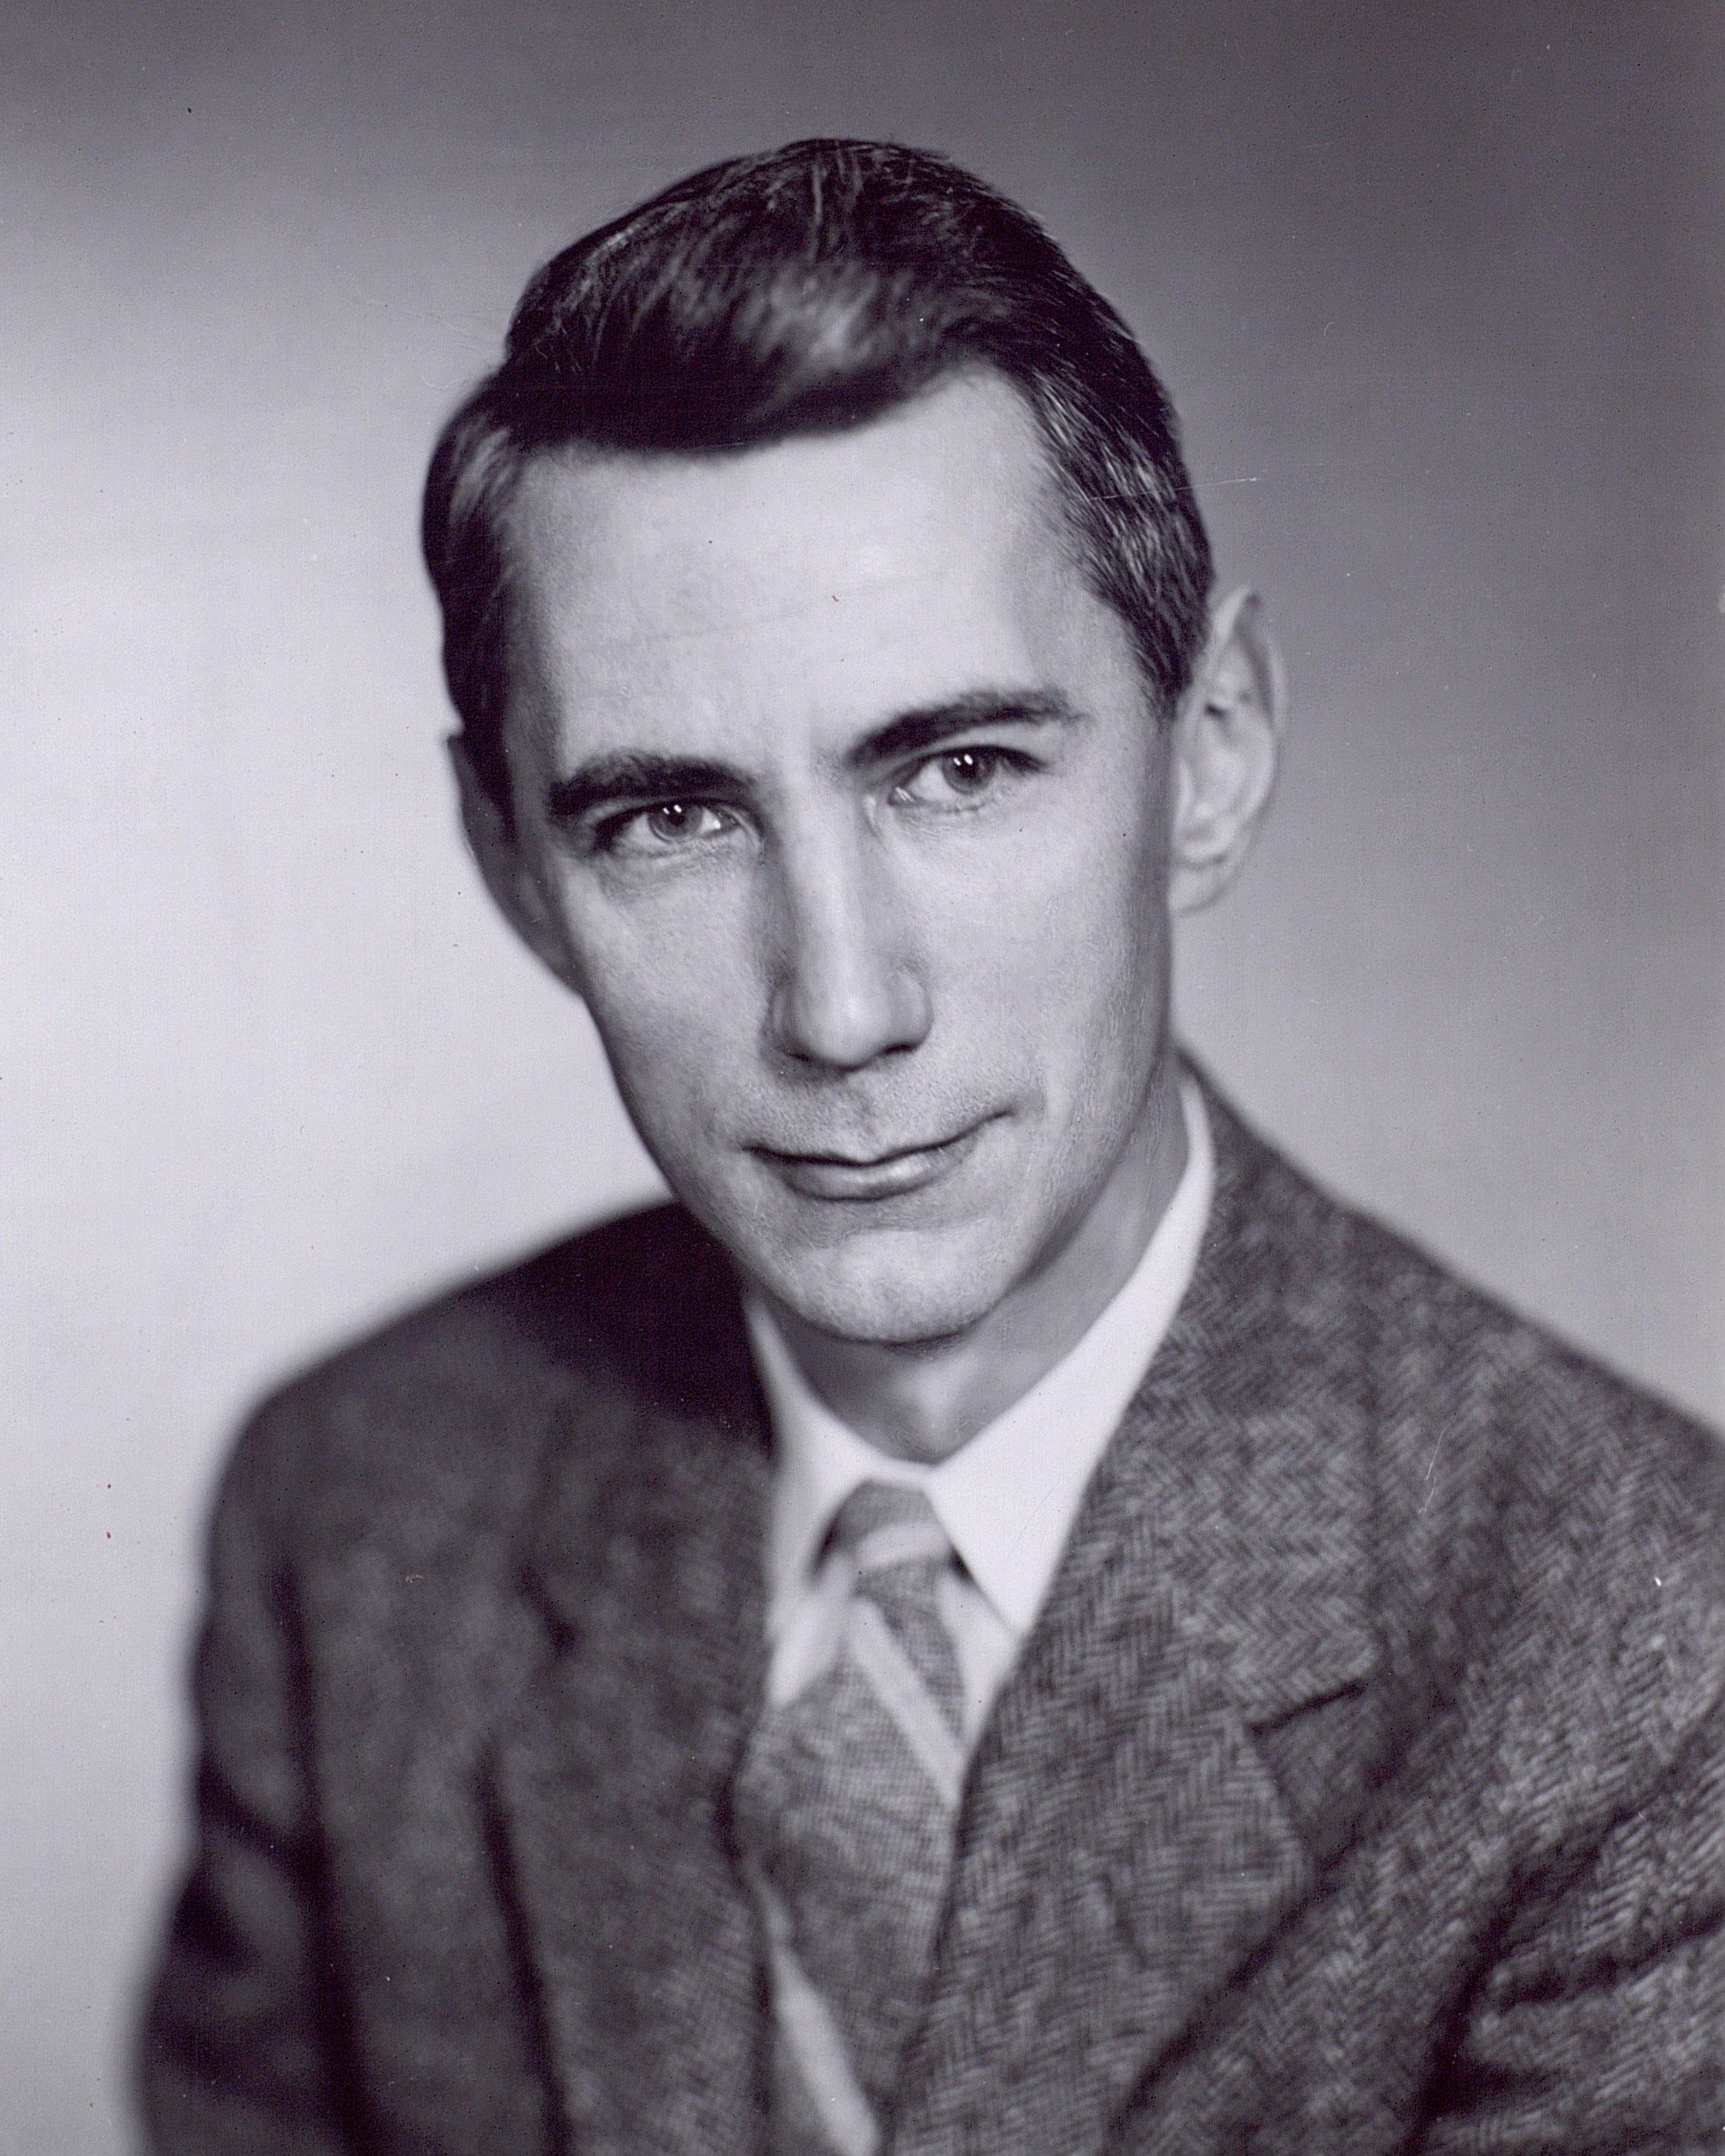
\includegraphics[width=0.25\linewidth]{images/Shannon.jpg}
    \caption{C.E.~Shannon. Source: By Unknown author - Tekniska Museet, CC BY 2.0, \url{https://commons.wikimedia.org/w/index.php?curid=144716444}}
    \label{Claude Shannon}
\end{figure}






Open: $\quad \mathrm{NEXP}\stackrel{?}{\subseteq}P/poly$ (note that by the time hierarchy theorem $\mathrm{EXP}\subsetneq P$; but in ``$\mathrm{NEXP}\stackrel{?}{\subseteq}P/poly$'' we consider NEXP which is \emph{uniform}, and P/poly which is \textit{non}-uniform).


\begin{theorem}
    [Shannon lower bound]
    For every $n>1$ exists a function $f:\{0,1\}^n \rightarrow\{0,1\}$ that cannot be computed by a circuit of size  $\le 2^n / 10 n$.
\end{theorem}

\begin{proof}[by counting method.]
\mbox{}\\

\begin{claim}
We can encode a boolean circuit of size $S$ with $9\cdot S \log S$ bits.
\end{claim}

\begin{proof}[Claim]
Using adjacency List:
\begin{figure}[H]
    \centering
    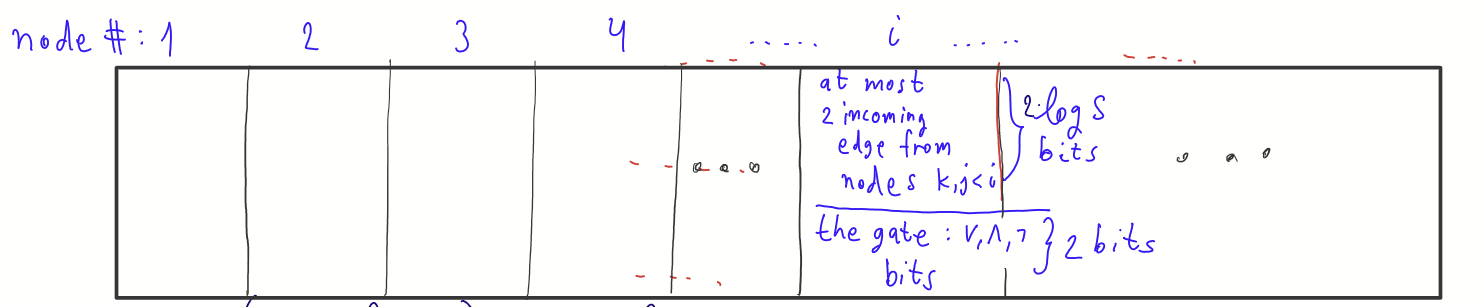
\includegraphics[width=1.1\linewidth]{images/shannon_table.png}
    \caption{Enter Caption}
    \label{fig:enter-label}
\end{figure}




We have:
$$
S \cdot(2+2 \log S) \leq 9 S \log S
.$$
(Actually, we have: 
$ 2S(\log S+1) = 2S(2 \log S) \leq 4 S \log S.
$)
\end{proof}

We now show that the number of circuits of size $\leq 2^n / 10 n$ is smaller than that of possible Boolean functions w/ $n$ inputs.
Thus, by the Pigeonhole Principle, there exists a Boolean function that cannot be computed by a circuit of size $\leq 2^n / 10 n$.

The number of circuits of size $S$ is bounded from above by the number of distinct codes of circuits of size $S$, which is
$$
\begin{aligned}
& \leq 2^{9 \cdot S \log S} \\
& =2^{\left(9 \cdot 2^{n / 10 n} \cdot \log \left(2^n / 10 n\right)\right)}=2^{\left(9 \cdot 2^n / 10 n \cdot(n-\log 10 n)\right)} \\
& \leq 2^{\frac{9 n}{10 n} \cdot 2^n}=2^{\frac{9}{10} \cdot 2^n} . 
\end{aligned}
$$
But this is 
less than $2^{2^n}$ the number of distinct Boolean functions $f:\{0,1\}^n\to\{0,1\}$. 
\end{proof}




Note: the reason we need to lower bound $2^n/10n$ circuits (and not $2^n/c$), is that encoding a circuit is super linear (i.e., $\Omega (\log n)$).




%%%%%%%%%%%%%%%%%%%%% chapter2.tex %%%%%%%%%%%%%%%%%%%%%%%%%%%%%%%%%
%
%  Monotone Circuits Lower bounds 
%
% Use this file as a template for your own input.
%
%%%%%%%%%%%%%%%%%%%%%%%% Springer-Verlag %%%%%%%%%%%%%%%%%%%%%%%%%%
%\motto{Use the template \emph{chapter.tex} to style the various elements of your chapter content.}





\chapter{Monotone Circuit Lower Bounds}
\label{sec:Razborov} % Always give a unique label
% use \chaptermark{}
% to alter or adjust the chapter heading in the running head


% Always give a unique label
% and use \ref{<label>} for cross-references
% and \cite{<label>} for bibliographic references
% use \sectionmark{}
% to alter or adjust the section heading in the running head

We've seen that proving that SAT is not in \Ppoly, i.e., can't be solved by polynomial-size circuits, implies that $\P \neq \NP$.
Due to the notorious difficulty of these questions, we are interested in proving \emph{weaker} lower bounds, namely, some lower bounds against restricted classes of circuits. 
Here, we study such a restricted circuit class: A boolean circuit without negation gates, i.e., monotone circuits.

\begin{definition}[Monotone circuit]
A Monotone circuit is a Boolean circuit that contains fan-in two gates AND and OR, but has \emph{no} NOT gates.
\end{definition}

This means in particular that monotone circuits can compute only monotone functions: a Boolean function is said to be monotone if increasing the number of ones in the input cannot flip the value of the function from 1 to 0. 

More precisely, for $\bar{x}, \bar{y} \in\{0,1\}^n$, write $\bar{x} \geqslant \bar{y}$ iff $ \forall i \in [n], x_i \geqslant y_i$, where $[n]$ denotes $\{1,\dots,n\}$. (Here, $x_i\ge y_i$ for Boolean $x_i,y_i$ means simply that $1\ge 0$ and $0\ge 0$, $1\ge 1$, while $0\not\ge 1$.)

\begin{definition}[Monotone function]
A Boolean function $f:\{0,1\}^n \rightarrow\{0,1\}$ is said to be  \emph{monotone} if $\forall \bar{x} \geq \bar{y}, f(\bar{x}) \geqslant f(y)$.
\end{definition}


Many NP problems are monotone, like CLIQUE:

Given an undirected graph $G=(V, E)$ with $n$ nodes, a $k$-clique in $G$ is a set $U\subseteq V$ of size $k$, st. every pair of nodes $u_1, u_2 \in U$ is connected by an edge (in $E$):

$$
 \forall u_1 \in u \forall u_2 \in u ( u \neq u_2\Rightarrow (u_1, u_2)\in E).
$$


Recall that a computational (decision) problem is a \emph{language}, namely an infinite set of finite strings over a finite alphabet (usually the alphabet $\{0,1\}$). Here, our language consists of all the strings that encode (in some natural way) an accepted graph, i.e., a $k$-clique with $n$ nodes.
The natural way to encode a graph in our case is this: a graph  $G=(V, E) $ with $n$ nodes, is encoded by $\binom{n}{2}$ input variables  $x_{ij}$, where the semantic of the encoding is: $x_{i j}=1$ iff $(i, j) \in E$. In other words, if the input variable $x_{ij}=1$,   our input graph contains the edge $(i,j)$, and otherwise it does not. 

We are interested in CLIQUE$(k, n)$ for a fixed $k$, as the following Boolean function: 
\begin{svgraybox}
The computational problem \textbf{CLIQUE$(k, n)$}: 

\textit{Input}: Undirected graph $G=(V,E)$ with $n$ nodes, and a number $k$ (given in unary, i.e., $1^k$).

\textit{Accept}: if the graph $G$ contains a $k$-clique. 

\textit{Reject}: otherwise.
\end{svgraybox}


 Note that $\operatorname{CLIQUE}(k, n)$ is a monotone function: If we add 1's to the input, we only \emph{increase} the chance it has a $k$-clique!
 
It is known that CLIQUE$(k,n)$ is NP-complete (see standard complexity textbooks; e.g., Papadimitriou 1994).


Since CLIQUE$(n, k)$ is a monotone (Boolean)
function we can compute it by a monotone Boolean circuit.

\begin{trailer}{Example of a monotone circuit computing CLIQUE$(n, k)$}
 ``Run" over all $\binom{n}{k} ~~ k$-sub-graphs in $G$, and check if at least one of those is a clique:

\begin{figure}
    \centering
    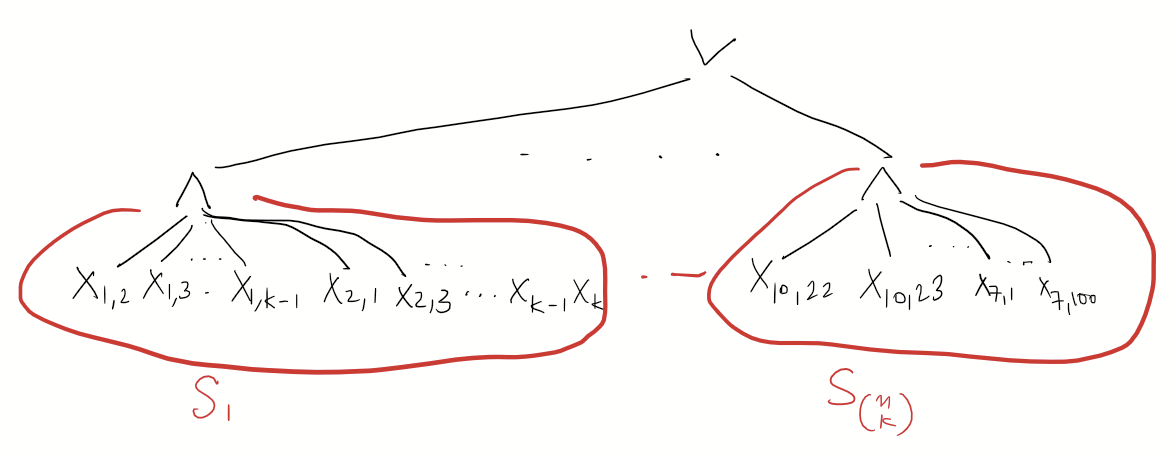
\includegraphics[width=0.75\linewidth]{images/k-clique-simple-circuit.png}
    \label{fig:enter-label}
\end{figure}

$S_1, S_2, \ldots, S_{\binom{n}{k}}$ are the $\binom{n}{k}$ subgraphs in $G$ each of size $k$.
Size of this circuit: $O\left(k^2 \cdot\binom{n}{k}\right)$.
We call such a circuit for computing $\operatorname{CLIQUE}  (n, k)$ consisting of a big $\lor$ of all $S_i$'s, each computed by $\land$'s of edges, a \textbf{\textit{crude-circuit}} for CLIQUE($n, k)$.
\end{trailer}



Notation: $CC\left(S_1, \ldots, S_{\binom{n}{k}}\right)$ is the crude circuit computing the $\lor$ of all subgraphs $S_1 \ldots S_{n\choose k }$. In general, we shall use different subgraphs: $CC\left(x_1, \ldots, x_m\right)$ for $x_i \subseteq V$ not necessarily of size $k$.


Note: When $k=w(\log n)$, $CC\left(S_1, \ldots, S_{\left(k_k\right)}\right)$ is of exponential size.
The following theorem shows this naive monotone circuit cannot be improved much:

\begin{figure}
    \centering
    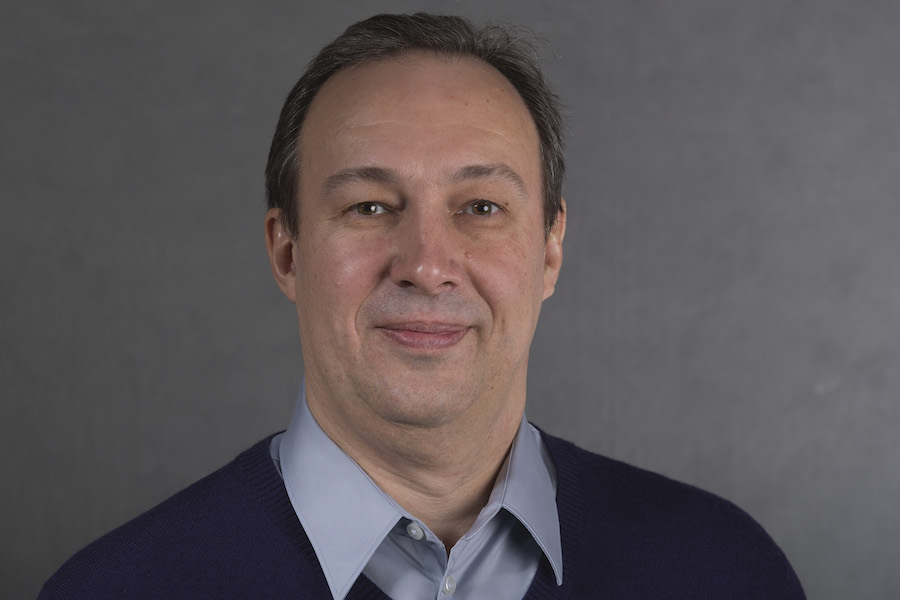
\includegraphics[width=0.25\linewidth]{images/RAZBOROV_Alexander.jpeg}
    \caption{Alexander Razborov}
    \label{fig:enter-label}
\end{figure}

\begin{svgraybox}
\begin{theorem}\label{thm:razborov}
    [Razborov] Let $k=\sqrt[4]{n}$. Then, every monotone circuit computing CLIQUE$(n, k)$ has size $2^{\Omega(\sqrt[8]{n})}$.
\end{theorem}
\end{svgraybox}
That is, exists a constant $c$ s.t. for large enough $n \in \mathbb{N}$, if $C_n$ computes CLIQUE$(n,k)$ then $\left|C_n\right| \geqslant 2^{c \cdot \sqrt[8]{n}}$.


%Recall: a crude circuit is a big OR of cliques, each computed as a big AND.



\paragraph{Approximation Method}

Here we provide an overview of the approach we take to prove \Cref{thm:razborov} which is called \emph{the approximation method}. Our exposition is taken from Papadimitriou's textbook \cite{Pap94}.
We shall describe a way of approximating any \textbf{monotone} circuit for $\operatorname{CLIQUE}({n}, {k})$ by a crude circuit, namely a big OR of cliques:

\begin{enumerate}
    
\item  Given a monotone circuit C , we shall construct a crude circuit ${CC}({X} 1, \ldots, {Xm})$ for some m and $\left|{X}_{{i}}\right| \leq l$ (for some $l$, all ${i}=1, \ldots, {m}$ ), that approximates $\operatorname{CLIQUE}({n}, {k})$ with \textbf{precision} that is dependent on the number of gates in $C$.

\item I.e., if the precision is not good, namely the crude circuit ${CC}({X} 1, \ldots, {Xm})$ for CLIQUE (n,k) we end up with makes \textit{many errors} on the CLIQUE ( $n, k$ ) function (i.e., says "NO" on an input that has a k-clique, and "YES" on an input that has no k-clique), it means that the circuit $C$ has \textit{many gates}, and vice versa.\label{it:approximation-b}

\item We show that every crude circuit ${CC}({X} 1, \ldots, {Xm})(|{X}_i| \leq l$ for some $l$, for all $i=1, \ldots, m$ ), ought to make \textit{exponentially many errors} on the function $\operatorname{CLIQUE}(n, k)$. From \ref{it:approximation-b} above we conclude that the number of gates in C was exponential.

\end{enumerate}


The \textbf{approximation} (i.e., construction of a crude circuit for CLIQUE(${n},{k})$ given the circuit $C$) will proceed in steps, one step for each gate of the monotone circuit:

\begin{enumerate}
    
\item If $C$ is a monotone circuit computing $\operatorname{CLIQUE}({n}, {k})$ we can \textit{approximate} any gate OR or AND in $C$ with a crude circuit.

\item Each such approximation step introduces rather few errors (false positives and false negatives).
\end{enumerate}


\section{Proof of monotone circuit lower bounds}

\begin{trailer}{Parameters \& notation}

Recall we want to compute CLIQUE$(n, k)$
with $n$ the number of nodes in the graph and $k$ the size of a clique within the graph. 
We set:
$$
k=\sqrt[4]{n}.
$$

\begin{svgraybox}\textbf{Goal}: Show that every monotone circuit computing $\operatorname{CLIQUE}(n,k)$ has size at least $2^{c \sqrt[8]{n}}$ for some constant $c$ (for sufficiently large $n$).
\end{svgraybox}

$$
\begin{aligned}
& l=\sqrt[8]{n} \\
& p \approx \sqrt[8]{n} \\
& M=(p-1)^l \cdot l! & \approx(\sqrt[8]{n}-1)^{\sqrt[8]{x}} \cdot(\sqrt[8]{n})! \\
& & \leq(\sqrt[4]{n})^{\sqrt[8]{n}}
\end{aligned}
$$


Each crude-circuit we use in the approximation is:

$$
C C\left(x_1, \ldots, x_m\right)
$$

for $m \leqslant M$ and $\left|X_i\right| \leqslant l, \forall i \in[m]$.

\end{trailer}

\bigskip 





- The approximation of the monotone circuit $C$ that computes $\operatorname{CLIQUE}(n, k)$ is done by induction on the size of $C$, ie., number of $\lor, \wedge$ gates in $C$.


- Comment: Such induction is also called ``Induction on the structure of $C$''.

- Such induction proceeds as follows: 


\para{Base Case} $|C|=1$, ie., $C$ consists of only a single input gate $g_{ij}$. Recall $g_{i j}$ is an input gate denoting whether $(i, j) \in E$, for $i, j \in V$.
That is, if there is an edge between $i$ and $j$ in the input graph $G$.

This is an easy case: We need to show a crude cat $\operatorname{CC}\left(X_1, \ldots, X_m\right) \mathrm{w} /$ $m \leqslant M$ and $\left|X_i\right| \leqslant l \quad \forall i \in[m]$ that
approximates $g_{i i}$ (without introducing too many errors; We shall count precisely the number of potential errors later).
But the circuit $C C(\{i, j\})=g_{i j}$ by definition. (Hence, no errors here!)


\para{Induction Step}
Given two crude circuits
$\operatorname{CC}(\mathcal X)$ and 
$\operatorname{CC}(\mathcal Y) 
$, with $\mathcal{X}=\{x_1, \ldots, x_m\}$, 
$\mathcal{Y}=\{y_1, \ldots, y_{m^{\prime}}\}$, $m\le M$, and $\left|x_i\right| \leq \ell $, for all $i$, $m'\le M $ and $\left|y_i\right| \leq \ell$, for all $i$.


We wish to construct another crude circuit  for computing $CC(\mathcal{X}) \vee CC(\mathcal{Y})$, and $\operatorname{CC}(\mathcal X) \wedge 
\operatorname{CC}(\mathcal Y)$.

\case{1}
$\lor$-gate.

Naive attempt: $\operatorname{CC}(\mathcal X)
\lor \operatorname{CC}(\mathcal Y)$ is approximated by $\operatorname{CC}(\mathcal X \cup \mathcal Y)$. That is, $\operatorname{CC}\left(x_1, \ldots, x_m, y_1, \ldots, y_m\right)$. At first glance this is a good solution because it does not introduce any errors (why?). But there is a problem: what if $m+m^{\prime}>M$?


Solution: We need to cleverly \emph{reduce} the number of sets $x_1, \ldots, x_m, y_1, \ldots, y_{m^{\prime}}$. To do this we use a combinatorial lemma called The Sunflower Lemma.

%%%%%%%%%%%%%%%%%%%%% chapter.tex %%%%%%%%%%%%%%%%%%%%%%%%%%%%%%%%%
%
% sample chapter
%
% Use this file as a template for your own input.
%
%%%%%%%%%%%%%%%%%%%%%%%% Springer-Verlag %%%%%%%%%%%%%%%%%%%%%%%%%%
%\motto{Use the template \emph{chapter.tex} to style the various elements of your chapter content.}
\chapter{Introduction}
\label{intro} % Always give a unique label
% use \chaptermark{}
% to alter or adjust the chapter heading in the running head

% \abstract*{Each chapter should be preceded by an abstract (no more than 200 words) that summarizes the content. The abstract will appear \textit{online} at \url{www.SpringerLink.com} and be available with unrestricted access. This allows unregistered users to read the abstract as a teaser for the complete chapter.
% Please use the 'starred' version of the new \texttt{abstract} command for typesetting the text of the online abstracts (cf. source file of this chapter template \texttt{abstract}) and include them with the source files of your manuscript. Use the plain \texttt{abstract} command if the abstract is also to appear in the printed version of the book.}

% \abstract{Each chapter should be preceded by an abstract (no more than 200 words) that summarizes the content. The abstract will appear \textit{online} at \url{www.SpringerLink.com} and be available with unrestricted access. This allows unregistered users to read the abstract as a teaser for the complete chapter. \newline\indent
% Please use the 'starred' version of the new \texttt{abstract} command for typesetting the text of the online abstracts (cf. source file of this chapter template \texttt{abstract}) and include them with the source files of your manuscript. Use the plain \texttt{abstract} command if the abstract is also to appear in the printed version of the book.}

\section{Section Heading}
\label{sec:1}
Use the template \emph{chapter.tex} together with the document class SVMono (monograph-type books) or SVMult (edited books) to style the various elements of your chapter content conformable to the Springer Nature layout.

\section{Section Heading}
\label{sec:2}
% Always give a unique label
% and use \ref{<label>} for cross-references
% and \cite{<label>} for bibliographic references
% use \sectionmark{}
% to alter or adjust the section heading in the running head
Instead of simply listing headings of different levels we recommend to let every heading be followed by at least a short passage of text. Furtheron please use the \LaTeX\ automatism for all your cross-references and citations.

Please note that the first line of text that follows a heading is not indented, whereas the first lines of all subsequent paragraphs are.

\eject

Use the standard \verb|equation| environment to typeset your equations, e.g.
%
\begin{equation}
a \times b = c\;,
\end{equation}
%
however, for multiline equations we recommend to use the \verb|eqnarray| environment\footnote{In physics texts please activate the class option \texttt{vecphys} to depict your vectors in \textbf{\itshape boldface-italic} type - as is customary for a wide range of physical subjects.}.
\begin{eqnarray}
\left|\nabla U_{\alpha}^{\mu}(y)\right| &\le&\frac1{d-\alpha}\int
\left|\nabla\frac1{|\xi-y|^{d-\alpha}}\right|\,d\mu(\xi) =
\int \frac1{|\xi-y|^{d-\alpha+1}} \,d\mu(\xi)\qquad  \\
&=&(d-\alpha+1) \int\limits_{d(y)}^\infty
\frac{\mu(B(y,r))}{r^{d-\alpha+2}}\,dr \le (d-\alpha+1)
\int\limits_{d(y)}^\infty \frac{r^{d-\alpha}}{r^{d-\alpha+2}}\,dr
\label{eq:01}
\end{eqnarray}

\enlargethispage{24pt}

\subsection{Subsection Heading}
\label{subsec:2}
Instead of simply listing headings of different levels we recommend to let every heading be followed by at least a short passage of text. Further on please use the \LaTeX\ automatism for all your cross-references\index{cross-references} and citations\index{citations} as has already been described in Sect.~\ref{sec:2}.

\begin{quotation}
Please do not use quotation marks when quoting texts! Simply use the \verb|quotation| environment -- it will automatically be rendered in the preferred layout.
\end{quotation}


\subsubsection{Subsubsection Heading}
Instead of simply listing headings of different levels we recommend to let every heading be followed by at least a short passage of text. Furtheron please use the \LaTeX\ automatism for all your cross-references and citations as has already been described in Sect.~\ref{subsec:2}, see also Fig.~\ref{fig:1}\footnote{If you copy text passages, figures, or tables from other works, you must obtain \textit{permission} from the copyright holder (usually the original publisher). Please enclose the signed permission with the manucript. The sources\index{permission to print} must be acknowledged either in the captions, as footnotes or in a separate section of the book.}

Please note that the first line of text that follows a heading is not indented, whereas the first lines of all subsequent paragraphs are.

% For figures use
%
\begin{figure}[b]
\sidecaption
% Use the relevant command for your figure-insertion program
% to insert the figure file.
% For example, with the option graphics use
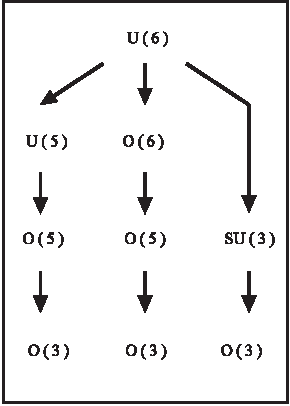
\includegraphics[scale=.65]{figure}
%
% If not, use
%\picplace{5cm}{2cm} % Give the correct figure height and width in cm
%
\caption{If the width of the figure is less than 7.8 cm use the \texttt{sidecapion} command to flush the caption on the left side of the page. If the figure is positioned at the top of the page, align the sidecaption with the top of the figure -- to achieve this you simply need to use the optional argument \texttt{[t]} with the \texttt{sidecaption} command}
\label{fig:1}       % Give a unique label
\end{figure}


\paragraph{Paragraph Heading} %
Instead of simply listing headings of different levels we recommend to let every heading be followed by at least a short passage of text. Furtheron please use the \LaTeX\ automatism for all your cross-references and citations as has already been described in Sect.~\ref{sec:2}.

Please note that the first line of text that follows a heading is not indented, whereas the first lines of all subsequent paragraphs are.

For typesetting numbered lists we recommend to use the \verb|enumerate| environment -- it will automatically render Springer's preferred layout.

\begin{enumerate}
\item{Livelihood and survival mobility are oftentimes coutcomes of uneven socioeconomic development.}
\begin{enumerate}
\item{Livelihood and survival mobility are oftentimes coutcomes of uneven socioeconomic development.}
\item{Livelihood and survival mobility are oftentimes coutcomes of uneven socioeconomic development.}
\end{enumerate}
\item{Livelihood and survival mobility are oftentimes coutcomes of uneven socioeconomic development.}
\end{enumerate}


\subparagraph{Subparagraph Heading} In order to avoid simply listing headings of different levels we recommend to let every heading be followed by at least a short passage of text. Use the \LaTeX\ automatism for all your cross-references and citations as has already been described in Sect.~\ref{sec:2}, see also Fig.~\ref{fig:2}.

Please note that the first line of text that follows a heading is not indented, whereas the first lines of all subsequent paragraphs are.

For unnumbered list we recommend to use the \verb|itemize| environment -- it will automatically render Springer's preferred layout.

\begin{itemize}
\item{Livelihood and survival mobility are oftentimes coutcomes of uneven socioeconomic development, cf. Table~\ref{tab:1}.}
\begin{itemize}
\item{Livelihood and survival mobility are oftentimes coutcomes of uneven socioeconomic development.}
\item{Livelihood and survival mobility are oftentimes coutcomes of uneven socioeconomic development.}
\end{itemize}
\item{Livelihood and survival mobility are oftentimes coutcomes of uneven socioeconomic development.}
\end{itemize}

\begin{figure}[t]
\sidecaption[t]
% Use the relevant command for your figure-insertion program
% to insert the figure file.
% For example, with the option graphics use
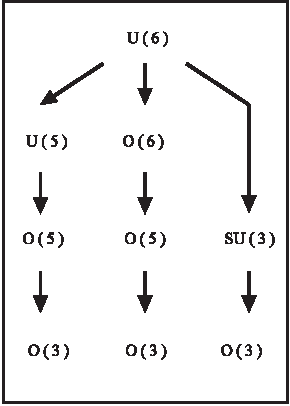
\includegraphics[scale=.65]{figure}
%
% If not, use
%\picplace{5cm}{2cm} % Give the correct figure height and width in cm
%
\caption{Please write your figure caption here}
\label{fig:2}       % Give a unique label
\end{figure}

\runinhead{Run-in Heading Boldface Version} Use the \LaTeX\ automatism for all your cross-references and citations as has already been described in Sect.~\ref{sec:2}.

\subruninhead{Run-in Heading Boldface and Italic Version} Use the \LaTeX\ automatism for all your cross-refer\-ences and citations as has already been described in Sect.~\ref{sec:2}\index{paragraph}.

\subsubruninhead{Run-in Heading Displayed Version} Use the \LaTeX\ automatism for all your cross-refer\-ences and citations as has already been described in Sect.~\ref{sec:2}\index{paragraph}.
% Use the \index{} command to code your index words
%
% For tables use
%
\begin{table}[!t]
\caption{Please write your table caption here}
\label{tab:1}       % Give a unique label
%
% For LaTeX tables use
%
\begin{tabular}{p{2cm}p{2.4cm}p{2cm}p{4.9cm}}
\hline\noalign{\smallskip}
Classes & Subclass & Length & Action Mechanism  \\
\noalign{\smallskip}\svhline\noalign{\smallskip}
Translation & mRNA$^a$  & 22 (19--25) & Translation repression, mRNA cleavage\\
Translation & mRNA cleavage & 21 & mRNA cleavage\\
Translation & mRNA  & 21--22 & mRNA cleavage\\
Translation & mRNA  & 24--26 & Histone and DNA Modification\\
\noalign{\smallskip}\hline\noalign{\smallskip}
\end{tabular}
$^a$ Table foot note (with superscript)
\end{table}
%
\section{Section Heading}
\label{sec:3}
% Always give a unique label
% and use \ref{<label>} for cross-references
% and \cite{<label>} for bibliographic references
% use \sectionmark{}
% to alter or adjust the section heading in the running head
Instead of simply listing headings of different levels we recommend to let every heading be followed by at least a short passage of text. Furtheron please use the \LaTeX\ automatism for all your cross-references and citations as has already been described in Sect.~\ref{sec:2}.

Please note that the first line of text that follows a heading is not indented, whereas the first lines of all subsequent paragraphs are.

If you want to list definitions or the like we recommend to use the Springer-enhanced \verb|description| environment -- it will automatically render Springer's preferred layout.

\begin{description}[Type 1]
\item[Type 1]{That addresses central themes pertainng to migration, health, and disease. In Sect.~\ref{sec:1}, Wilson discusses the role of human migration in infectious disease distributions and patterns.}
\item[Type 2]{That addresses central themes pertainng to migration, health, and disease. In Sect.~\ref{subsec:2}, Wilson discusses the role of human migration in infectious disease distributions and patterns.}
\end{description}

\subsection{Subsection Heading} %
In order to avoid simply listing headings of different levels we recommend to let every heading be followed by at least a short passage of text. Use the \LaTeX\ automatism for all your cross-references and citations citations as has already been described in Sect.~\ref{sec:2}.

Please note that the first line of text that follows a heading is not indented, whereas the first lines of all subsequent paragraphs are.

\begin{svgraybox}
If you want to emphasize complete paragraphs of texts we recommend to use the newly defined Springer class option \verb|graybox| and the newly defined environment \verb|svgraybox|. This will produce a 15 percent screened box 'behind' your text.

If you want to emphasize complete paragraphs of texts we recommend to use the newly defined Springer class option and environment \verb|svgraybox|. This will produce a 15 percent screened box 'behind' your text.
\end{svgraybox}


\subsubsection{Subsubsection Heading}
Instead of simply listing headings of different levels we recommend to let every heading be followed by at least a short passage of text. Furtheron please use the \LaTeX\ automatism for all your cross-references and citations as has already been described in Sect.~\ref{sec:2}.

Please note that the first line of text that follows a heading is not indented, whereas the first lines of all subsequent paragraphs are.

\begin{theorem}
Theorem text goes here.
\end{theorem}
%
% or
%
\begin{definition}
Definition text goes here.
\end{definition}

\begin{proof}
%\smartqed
Proof text goes here.
%\qed
\end{proof}

\paragraph{Paragraph Heading} %
Instead of simply listing headings of different levels we recommend to let every heading be followed by at least a short passage of text. Furtheron please use the \LaTeX\ automatism for all your cross-references and citations as has already been described in Sect.~\ref{sec:2}.

Note that the first line of text that follows a heading is not indented, whereas the first lines of all subsequent paragraphs are.
%
% For built-in environments use
%
\begin{theorem}
Theorem text goes here.
\end{theorem}
%
\begin{definition}
Definition text goes here.
\end{definition}
%
\begin{proof}
%\smartqed
Proof text goes here.
%\qed
\end{proof}
%
%
\begin{trailer}{Trailer Head}
If you want to emphasize complete paragraphs of texts in an \verb|Trailer Head| we recommend to
use  \begin{verbatim}\begin{trailer}{Trailer Head}
...
\end{trailer}\end{verbatim}
\end{trailer}
%
\begin{question}{Questions}
If you want to emphasize complete paragraphs of texts in an \verb|Questions| we recommend to
use  \begin{verbatim}\begin{question}{Questions}
...
\end{question}\end{verbatim}
\end{question}
%
%
\begin{important}{Important}
If you want to emphasize complete paragraphs of texts in an \verb|Important| we recommend to
use  \begin{verbatim}\begin{important}{Important}
...
\end{important}\end{verbatim}
\end{important}
%
\clearpage
\begin{warning}{Attention}
If you want to emphasize complete paragraphs of texts in an \verb|Attention| we recommend to
use  \begin{verbatim}\begin{warning}{Attention}
...
\end{warning}\end{verbatim}
\end{warning}

\begin{programcode}{Program Code}
If you want to emphasize complete paragraphs of texts in an \verb|Program Code| we recommend to
use

\verb|\begin{programcode}{Program Code}|

\verb|\begin{verbatim}...\end{verbatim}|

\verb|\end{programcode}|

\end{programcode}
%
\begin{tips}{Tips}
If you want to emphasize complete paragraphs of texts in an \verb|Tips| we recommend to
use  \begin{verbatim}\begin{tips}{Tips}
...
\end{tips}\end{verbatim}
\end{tips}
%
%
\begin{overview}{Overview}
If you want to emphasize complete paragraphs of texts in an \verb|Overview| we recommend to
use  \begin{verbatim}\begin{overview}{Overview}
...
\end{overview}\end{verbatim}
\end{overview}
\clearpage
\begin{backgroundinformation}{Background Information}
If you want to emphasize complete paragraphs of texts in an \verb|Background|
\verb|Information| we recommend to
use

\verb|\begin{backgroundinformation}{Background Information}|

\verb|...|

\verb|\end{backgroundinformation}|
\end{backgroundinformation}
\begin{legaltext}{Legal Text}
If you want to emphasize complete paragraphs of texts in an \verb|Legal Text| we recommend to
use  \begin{verbatim}\begin{legaltext}{Legal Text}
...
\end{legaltext}\end{verbatim}
\end{legaltext}
%
\begin{acknowledgement}
If you want to include acknowledgments of assistance and the like at the end of an individual chapter please use the \verb|acknowledgement| environment -- it will automatically render Springer's preferred layout.
\end{acknowledgement}
%
\section*{Appendix}
\addcontentsline{toc}{section}{Appendix}
%
When placed at the end of a chapter or contribution (as opposed to at the end of the book), the numbering of tables, figures, and equations in the appendix section continues on from that in the main text. Hence please \textit{do not} use the \verb|appendix| command when writing an appendix at the end of your chapter or contribution. If there is only one the appendix is designated ``Appendix'', or ``Appendix 1'', or ``Appendix 2'', etc. if there is more than one.

\begin{equation}
a \times b = c
\end{equation}
% Problems or Exercises should be sorted chapterwise
\section*{Problems}
\addcontentsline{toc}{section}{Problems}
%
% Use the following environment.
% Don't forget to label each problem;
% the label is needed for the solutions' environment
\begin{prob}
\label{prob1}
A given problem or Excercise is described here. The
problem is described here. The problem is described here.
\end{prob}

\begin{prob}
\label{prob2}
\textbf{Problem Heading}\\
(a) The first part of the problem is described here.\\
(b) The second part of the problem is described here.
\end{prob}

%%%%%%%%%%%%%%%%%%%%%%%% referenc.tex %%%%%%%%%%%%%%%%%%%%%%%%%%%%%%
% sample references
% %
% Use this file as a template for your own input.
%
%%%%%%%%%%%%%%%%%%%%%%%% Springer-Verlag %%%%%%%%%%%%%%%%%%%%%%%%%%
%
% BibTeX users please use
% \bibliographystyle{}
% \bibliography{}
%
\biblstarthook{In view of the parallel print and (chapter-wise) online publication of your book at \url{www.springerlink.com} it has been decided that -- as a genreral rule --  references should be sorted chapter-wise and placed at the end of the individual chapters. However, upon agreement with your contact at Springer you may list your references in a single seperate chapter at the end of your book. Deactivate the class option \texttt{sectrefs} and the \texttt{thebibliography} environment will be put out as a chapter of its own.\\\indent
References may be \textit{cited} in the text either by number (preferred) or by author/year.\footnote{Make sure that all references from the list are cited in the text. Those not cited should be moved to a separate \textit{Further Reading} section or chapter.} If the citatiion in the text is numbered, the reference list should be arranged in ascending order. If the citation in the text is author/year, the reference list should be \textit{sorted} alphabetically and if there are several works by the same author, the following order should be used:
\begin{enumerate}
\item all works by the author alone, ordered chronologically by year of publication
\item all works by the author with a coauthor, ordered alphabetically by coauthor
\item all works by the author with several coauthors, ordered chronologically by year of publication.
\end{enumerate}
The \textit{styling} of references\footnote{Always use the standard abbreviation of a journal's name according to the ISSN \textit{List of Title Word Abbreviations}, see \url{http://www.issn.org/en/node/344}} depends on the subject of your book:
\begin{itemize}
\item The \textit{two} recommended styles for references in books on \textit{mathematical, physical, statistical and computer sciences} are depicted in ~\cite{science-contrib, science-online, science-mono, science-journal, science-DOI} and ~\cite{phys-online, phys-mono, phys-journal, phys-DOI, phys-contrib}.
\item Examples of the most commonly used reference style in books on \textit{Psychology, Social Sciences} are~\cite{psysoc-mono, psysoc-online,psysoc-journal, psysoc-contrib, psysoc-DOI}.
\item Examples for references in books on \textit{Humanities, Linguistics, Philosophy} are~\cite{humlinphil-journal, humlinphil-contrib, humlinphil-mono, humlinphil-online, humlinphil-DOI}.
\item Examples of the basic Springer style used in publications on a wide range of subjects such as \textit{Computer Science, Economics, Engineering, Geosciences, Life Sciences, Medicine, Biomedicine} are ~\cite{basic-contrib, basic-online, basic-journal, basic-DOI, basic-mono}. 
\end{itemize}
}

\begin{thebibliography}{99.}%
% and use \bibitem to create references.
%
% Use the following syntax and markup for your references if 
% the subject of your book is from the field 
% "Mathematics, Physics, Statistics, Computer Science"
%
% Contribution 
\bibitem{science-contrib} Broy, M.: Software engineering --- from auxiliary to key technologies. In: Broy, M., Dener, E. (eds.) Software Pioneers, pp. 10-13. Springer, Heidelberg (2002)
%
% Online Document
\bibitem{science-online} Dod, J.: Effective substances. In: The Dictionary of Substances and Their Effects. Royal Society of Chemistry (1999) Available via DIALOG. \\
\url{http://www.rsc.org/dose/title of subordinate document. Cited 15 Jan 1999}
%
% Monograph
\bibitem{science-mono} Geddes, K.O., Czapor, S.R., Labahn, G.: Algorithms for Computer Algebra. Kluwer, Boston (1992) 
%
% Journal article
\bibitem{science-journal} Hamburger, C.: Quasimonotonicity, regularity and duality for nonlinear systems of partial differential equations. Ann. Mat. Pura. Appl. \textbf{169}, 321--354 (1995)
%
% Journal article by DOI
\bibitem{science-DOI} Slifka, M.K., Whitton, J.L.: Clinical implications of dysregulated cytokine production. J. Mol. Med. (2000) doi: 10.1007/s001090000086 
%
\bigskip

% Use the following (APS) syntax and markup for your references if 
% the subject of your book is from the field 
% "Mathematics, Physics, Statistics, Computer Science"
%
% Online Document
\bibitem{phys-online} J. Dod, in \textit{The Dictionary of Substances and Their Effects}, Royal Society of Chemistry. (Available via DIALOG, 1999), 
\url{http://www.rsc.org/dose/title of subordinate document. Cited 15 Jan 1999}
%
% Monograph
\bibitem{phys-mono} H. Ibach, H. L\"uth, \textit{Solid-State Physics}, 2nd edn. (Springer, New York, 1996), pp. 45-56 
%
% Journal article
\bibitem{phys-journal} S. Preuss, A. Demchuk Jr., M. Stuke, Appl. Phys. A \textbf{61}
%
% Journal article by DOI
\bibitem{phys-DOI} M.K. Slifka, J.L. Whitton, J. Mol. Med., doi: 10.1007/s001090000086
%
% Contribution 
\bibitem{phys-contrib} S.E. Smith, in \textit{Neuromuscular Junction}, ed. by E. Zaimis. Handbook of Experimental Pharmacology, vol 42 (Springer, Heidelberg, 1976), p. 593
%
\bigskip
%
% Use the following syntax and markup for your references if 
% the subject of your book is from the field 
% "Psychology, Social Sciences"
%
%
% Monograph
\bibitem{psysoc-mono} Calfee, R.~C., \& Valencia, R.~R. (1991). \textit{APA guide to preparing manuscripts for journal publication.} Washington, DC: American Psychological Association.
%
% Online Document
\bibitem{psysoc-online} Dod, J. (1999). Effective substances. In: The dictionary of substances and their effects. Royal Society of Chemistry. Available via DIALOG. \\
\url{http://www.rsc.org/dose/Effective substances.} Cited 15 Jan 1999.
%
% Journal article
\bibitem{psysoc-journal} Harris, M., Karper, E., Stacks, G., Hoffman, D., DeNiro, R., Cruz, P., et al. (2001). Writing labs and the Hollywood connection. \textit{J Film} Writing, 44(3), 213--245.
%
% Contribution 
\bibitem{psysoc-contrib} O'Neil, J.~M., \& Egan, J. (1992). Men's and women's gender role journeys: Metaphor for healing, transition, and transformation. In B.~R. Wainrig (Ed.), \textit{Gender issues across the life cycle} (pp. 107--123). New York: Springer.
%
% Journal article by DOI
\bibitem{psysoc-DOI}Kreger, M., Brindis, C.D., Manuel, D.M., Sassoubre, L. (2007). Lessons learned in systems change initiatives: benchmarks and indicators. \textit{American Journal of Community Psychology}, doi: 10.1007/s10464-007-9108-14.
%
%
% Use the following syntax and markup for your references if 
% the subject of your book is from the field 
% "Humanities, Linguistics, Philosophy"
%
\bigskip
%
% Journal article
\bibitem{humlinphil-journal} Alber John, Daniel C. O'Connell, and Sabine Kowal. 2002. Personal perspective in TV interviews. \textit{Pragmatics} 12:257--271
%
% Contribution 
\bibitem{humlinphil-contrib} Cameron, Deborah. 1997. Theoretical debates in feminist linguistics: Questions of sex and gender. In \textit{Gender and discourse}, ed. Ruth Wodak, 99--119. London: Sage Publications.
%
% Monograph
\bibitem{humlinphil-mono} Cameron, Deborah. 1985. \textit{Feminism and linguistic theory.} New York: St. Martin's Press.
%
% Online Document
\bibitem{humlinphil-online} Dod, Jake. 1999. Effective substances. In: The dictionary of substances and their effects. Royal Society of Chemistry. Available via DIALOG. \\
http://www.rsc.org/dose/title of subordinate document. Cited 15 Jan 1999
%
% Journal article by DOI
\bibitem{humlinphil-DOI} Suleiman, Camelia, Daniel C. O'Connell, and Sabine Kowal. 2002. `If you and I, if we, in this later day, lose that sacred fire...': Perspective in political interviews. \textit{Journal of Psycholinguistic Research}. doi: 10.1023/A:1015592129296.
%
%
%
\bigskip
%
%
% Use the following syntax and markup for your references if 
% the subject of your book is from the field 
% "Computer Science, Economics, Engineering, Geosciences, Life Sciences"
%
%
% Contribution 
\bibitem{basic-contrib} Brown B, Aaron M (2001) The politics of nature. In: Smith J (ed) The rise of modern genomics, 3rd edn. Wiley, New York 
%
% Online Document
\bibitem{basic-online} Dod J (1999) Effective Substances. In: The dictionary of substances and their effects. Royal Society of Chemistry. Available via DIALOG. \\
\url{http://www.rsc.org/dose/title of subordinate document. Cited 15 Jan 1999}
%
% Journal article by DOI
\bibitem{basic-DOI} Slifka MK, Whitton JL (2000) Clinical implications of dysregulated cytokine production. J Mol Med, doi: 10.1007/s001090000086
%
% Journal article
\bibitem{basic-journal} Smith J, Jones M Jr, Houghton L et al (1999) Future of health insurance. N Engl J Med 965:325--329
%
% Monograph
\bibitem{basic-mono} South J, Blass B (2001) The future of modern genomics. Blackwell, London 
%
\end{thebibliography}


%%%%%%%%%%%%%%%%%%%%%% appendix.tex %%%%%%%%%%%%%%%%%%%%%%%%%%%%%%%%%
%
% sample appendix
%
% Use this file as a template for your own input.
%
%%%%%%%%%%%%%%%%%%%%%%%% Springer-Verlag %%%%%%%%%%%%%%%%%%%%%%%%%%

\appendix
\motto{All's well that ends well}
\chapter{Chapter Heading}
\label{introA} % Always give a unique label
% use \chaptermark{}
% to alter or adjust the chapter heading in the running head

Use the template \emph{appendix.tex} together with the Springer document class SVMono (monograph-type books) or SVMult (edited books) to style appendix of your book.


\section{Section Heading}
\label{sec:A1}
% Always give a unique label
% and use \ref{<label>} for cross-references
% and \cite{<label>} for bibliographic references
% use \sectionmark{}
% to alter or adjust the section heading in the running head
Instead of simply listing headings of different levels we recommend to let every heading be followed by at least a short passage of text. Furtheron please use the \LaTeX\ automatism for all your cross-references and citations.


\subsection{Subsection Heading}
\label{sec:A2}
Instead of simply listing headings of different levels we recommend to let every heading be followed by at least a short passage of text. Furtheron please use the \LaTeX\ automatism for all your cross-references and citations as has already been described in Sect.~\ref{sec:A1}.

For multiline equations we recommend to use the \verb|eqnarray| environment.
\begin{eqnarray}
\vec{a}\times\vec{b}=\vec{c} \nonumber\\
\vec{a}\times\vec{b}=\vec{c}
\label{eq:A01}
\end{eqnarray}

\subsubsection{Subsubsection Heading}
Instead of simply listing headings of different levels we recommend to let every heading be followed by at least a short passage of text. Furtheron please use the \LaTeX\ automatism for all your cross-references and citations as has already been described in Sect.~\ref{sec:A2}.

Please note that the first line of text that follows a heading is not indented, whereas the first lines of all subsequent paragraphs are.

% For figures use
%
\begin{figure}[t]
\sidecaption[t]
%\centering
% Use the relevant command for your figure-insertion program
% to insert the figure file.
% For example, with the option graphics use
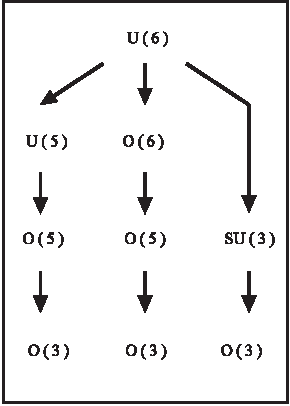
\includegraphics[scale=.65]{figure}
%
% If not, use
%\picplace{5cm}{2cm} % Give the correct figure height and width in cm
%
\caption{Please write your figure caption here}
\label{fig:A1}       % Give a unique label
\end{figure}

% For tables use
%
\begin{table}
\caption{Please write your table caption here}
\label{tab:A1}       % Give a unique label
%
% For LaTeX tables use
%
\begin{tabular}{p{2cm}p{2.4cm}p{2cm}p{4.9cm}}
\hline\noalign{\smallskip}
Classes & Subclass & Length & Action Mechanism  \\
\noalign{\smallskip}\hline\noalign{\smallskip}
Translation & mRNA$^a$  & 22 (19--25) & Translation repression, mRNA cleavage\\
Translation & mRNA cleavage & 21 & mRNA cleavage\\
Translation & mRNA  & 21--22 & mRNA cleavage\\
Translation & mRNA  & 24--26 & Histone and DNA Modification\\
\noalign{\smallskip}\hline\noalign{\smallskip}
\end{tabular}
$^a$ Table foot note (with superscript)
\end{table}
%


\backmatter%%%%%%%%%%%%%%%%%%%%%%%%%%%%%%%%%%%%%%%%%%%%%%%%%%%%%%%
%%%%%%%%%%%%%%%%%%%%%%%acronym.tex%%%%%%%%%%%%%%%%%%%%%%%%%%%%%%%%%%%%%%%%%
% sample list of acronyms
%
% Use this file as a template for your own input.
%
%%%%%%%%%%%%%%%%%%%%%%%% Springer %%%%%%%%%%%%%%%%%%%%%%%%%%

\Extrachap{Glossary}


Use the template \emph{glossary.tex} together with the Springer document class SVMono (monograph-type books) or SVMult (edited books) to style your glossary\index{glossary} in the Springer layout.


\runinhead{glossary term} Write here the description of the glossary term. Write here the description of the glossary term. Write here the description of the glossary term.

\runinhead{glossary term} Write here the description of the glossary term. Write here the description of the glossary term. Write here the description of the glossary term.

\runinhead{glossary term} Write here the description of the glossary term. Write here the description of the glossary term. Write here the description of the glossary term.

\runinhead{glossary term} Write here the description of the glossary term. Write here the description of the glossary term. Write here the description of the glossary term.

\runinhead{glossary term} Write here the description of the glossary term. Write here the description of the glossary term. Write here the description of the glossary term.
%
\Extrachap{Solutions}

\section*{Problems of Chapter~\ref{intro}}

\begin{sol}{prob1}
The solution\index{problems}\index{solutions} is revealed here.
\end{sol}


\begin{sol}{prob2}
\textbf{Problem Heading}\\
(a) The solution of first part is revealed here.\\
(b) The solution of second part is revealed here.
\end{sol}


%\printindex

%%%%%%%%%%%%%%%%%%%%%%%%%%%%%%%%%%%%%%%%%%%%%%%%%%%%%%%%%%%%%%%%%%%%%%

\end{document}





